% !TeX root = ../main.tex
\section{Introduction}
\label{sec:introduction}
Music-to-text choreography takes a musical recording and produces a
timed score of movements. Such a score makes compositional decisions
inspectable and editable before performance or rendering. Music-conditioned
dance generators synthesize motion sequences~\cite{aistpp,bailando,edge};
we study the textual planning interface, where movement content, its
ordering, and its development across a song must be stated explicitly.

This task presents three requirements. First, descriptions must specify
actionable movements rather than merely characterize the music. Training
them requires movement supervision with traceable source evidence.
Second, locally plausible actions must form a composition: independent
short-clip predictions do not determine transitions, motif recurrence,
or progression over an entire song. Third, evaluation must accommodate
multiple valid dances for the same music. Agreement with one recorded
dance therefore measures only part of the task; musical response and
whole-song organization require separate assessment.

We address these requirements with \method, which decouples local movement
prediction from global composition. A dedicated short-clip model provides
movement proposals. A stateful harness groups two to four musical bars
into duration-aware units and composes them using a segment outline,
shared musical evidence, a global dance-style condition, and accepted
history. Motif memory tracks recurrence and variation. Schedule validation
precedes commitment, while bounded revision targets repetitive action
spans and preserves their temporal scaffold. The outer planner operates
with fixed model weights.

The framework delivers an evidence-linked annotation resource and
construction pipeline, a task-specific model trained by supervised
fine-tuning, a compositional harness, and an evaluation protocol with
six local and three whole-song dimensions. Current experimental captions
refine 2D rule logs using GPT-6.1-sol; the implemented geometry-aware 3D
annotation route remains an extension. The evaluation protocol requests
explicit textual and musical evidence, separating reference agreement
from judgments of choreography quality.

On a frozen 2,000-clip panel, the adapted model achieves 30.80 ROUGE-L,
compared with 14.99 for the best evaluated general audio-language baseline
on this metric. These results characterize reference agreement;
music-conditioned quality requires separate assessment. Whole-song results use the historical
fixed-window harness; controlled comparisons of the latest bar-aligned
agents and independent audio-grounded assessment remain prospective.

% !TeX root = ../main.tex
\begin{figure*}[t]
\centering
\ifdefined\OverviewDataBenchmark
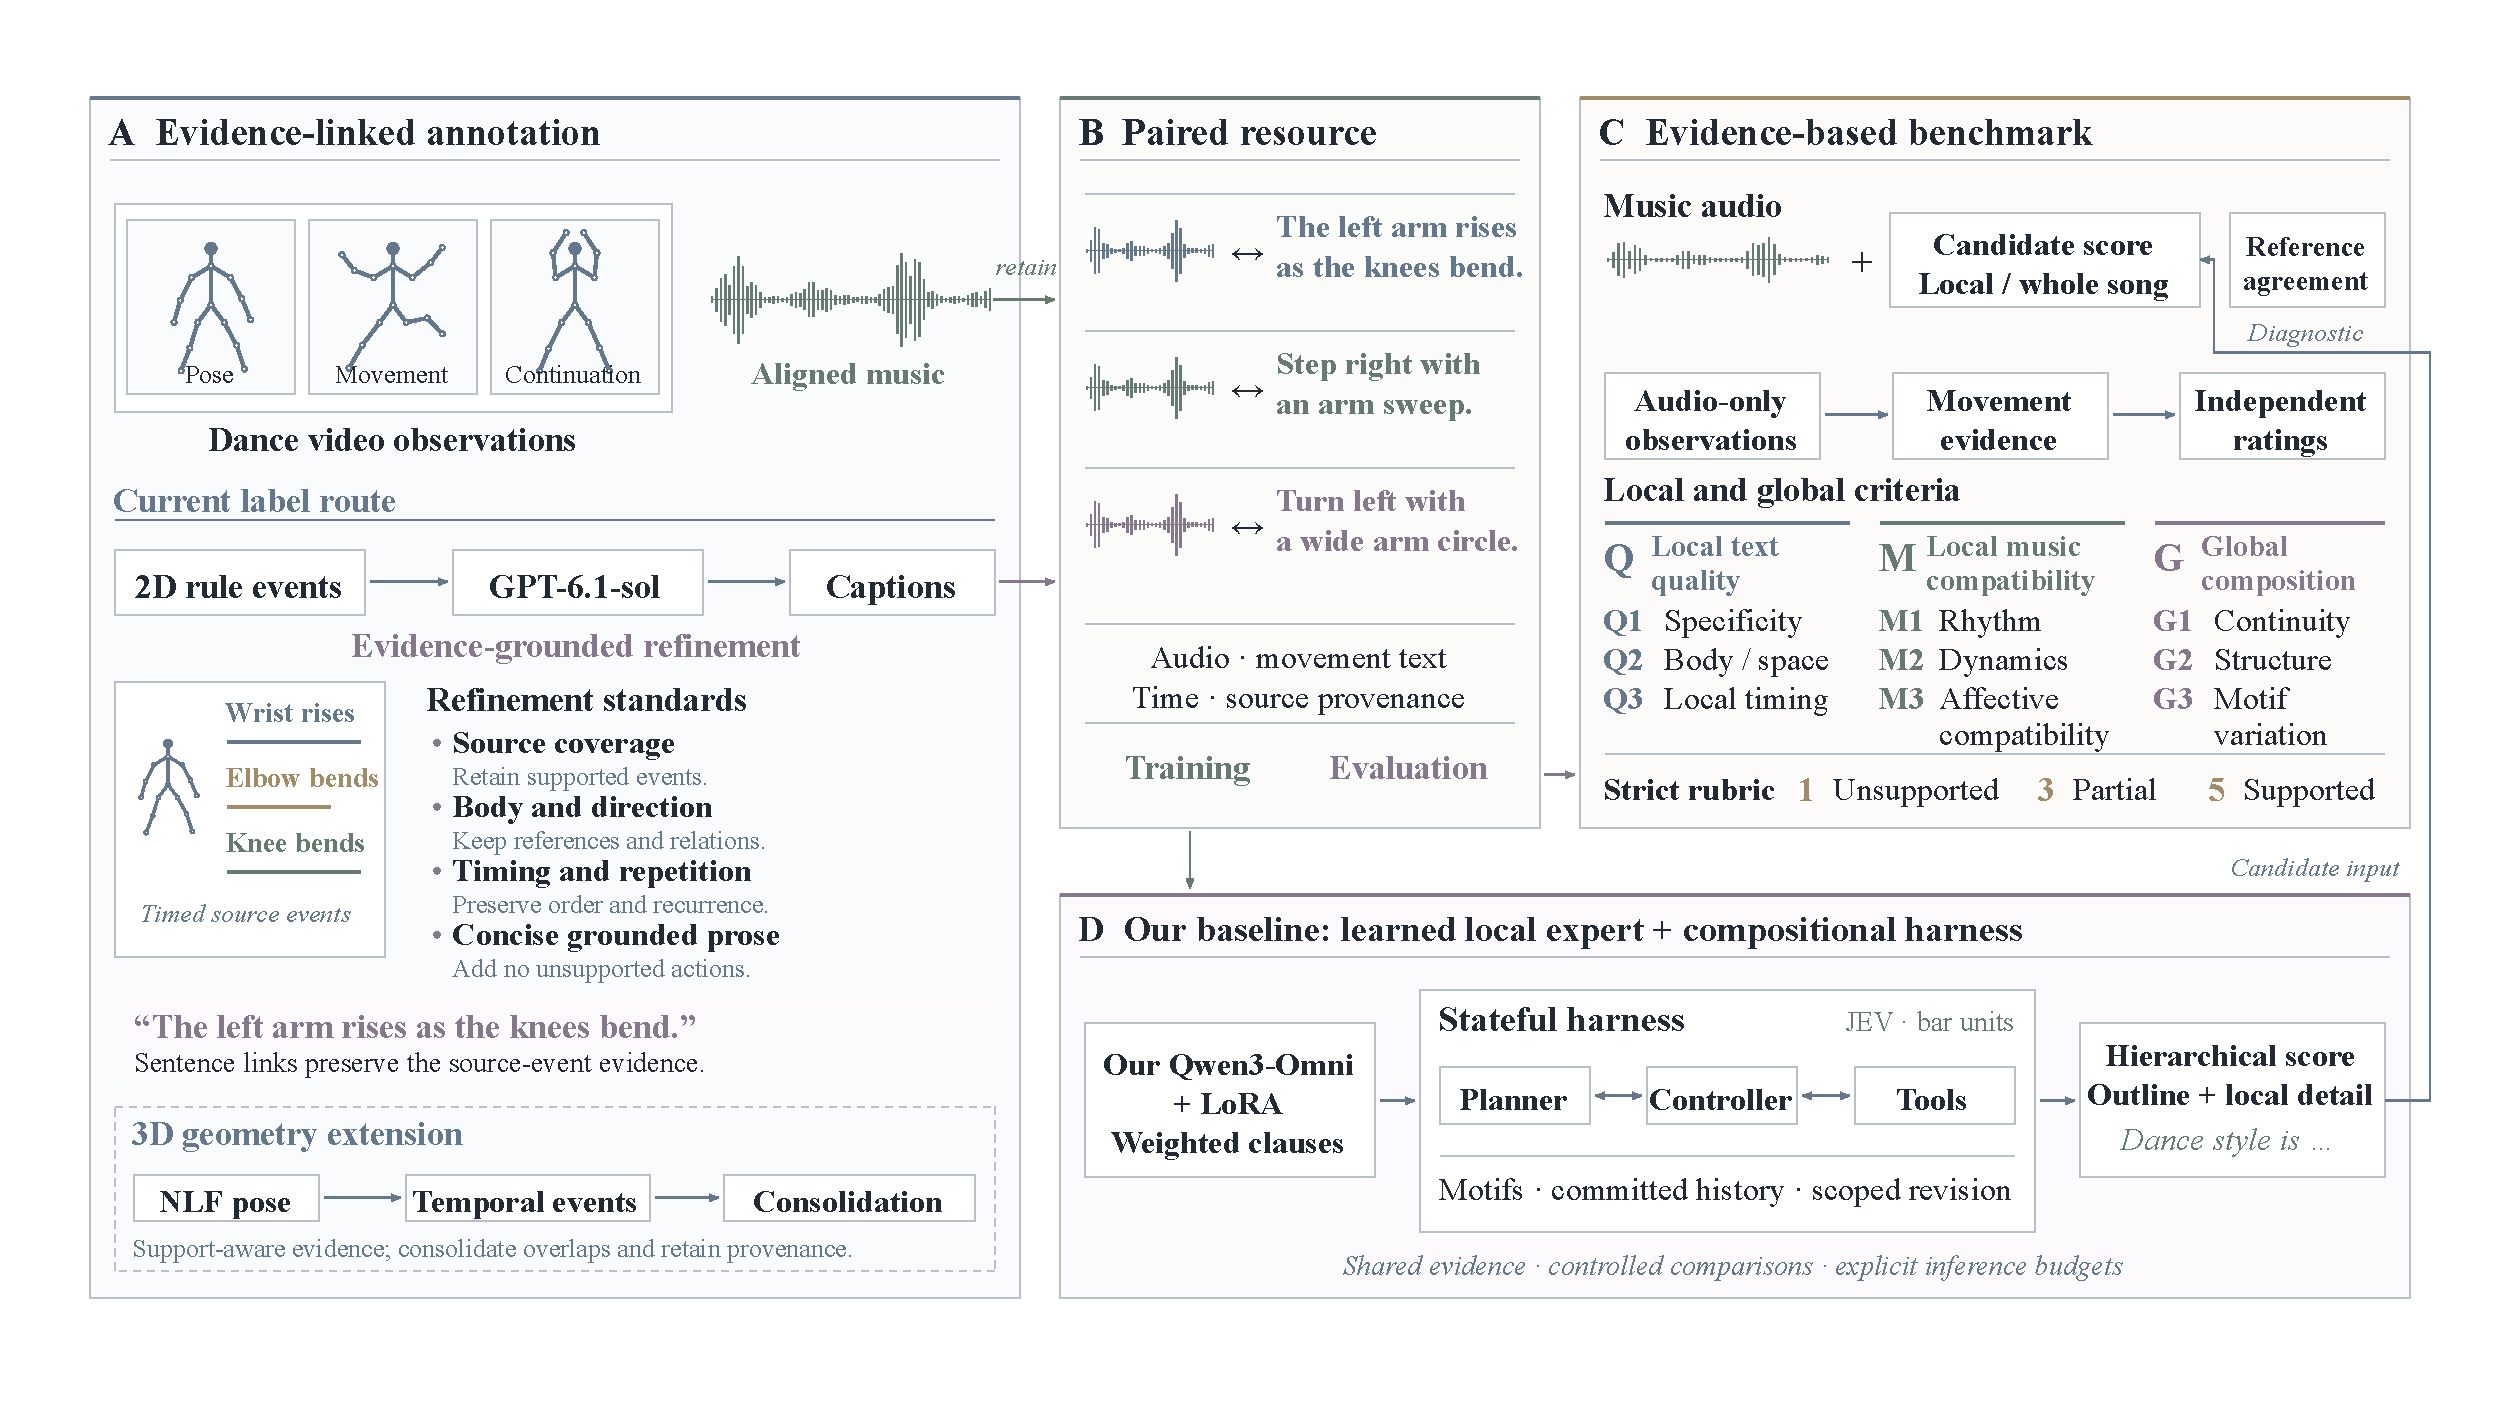
\includegraphics[width=\textwidth]{figures/revision_20261117/paper/overview_benchmark.pdf}
\caption{\textbf{Data, benchmark, and baseline in \method.}
Evidence-linked captions retain movement provenance and paired music.
Current labels follow the 2D rule-event route; the dashed 3D route
depicts the geometry extension. The trained local expert and stateful
harness provide a baseline for assessing local movement, musical
response, and whole-song composition. The proposed protocol uses audio
and quoted movement evidence; calibration remains pending.
Media, score snippets, and rubric anchors are schematic illustrations.}
\else
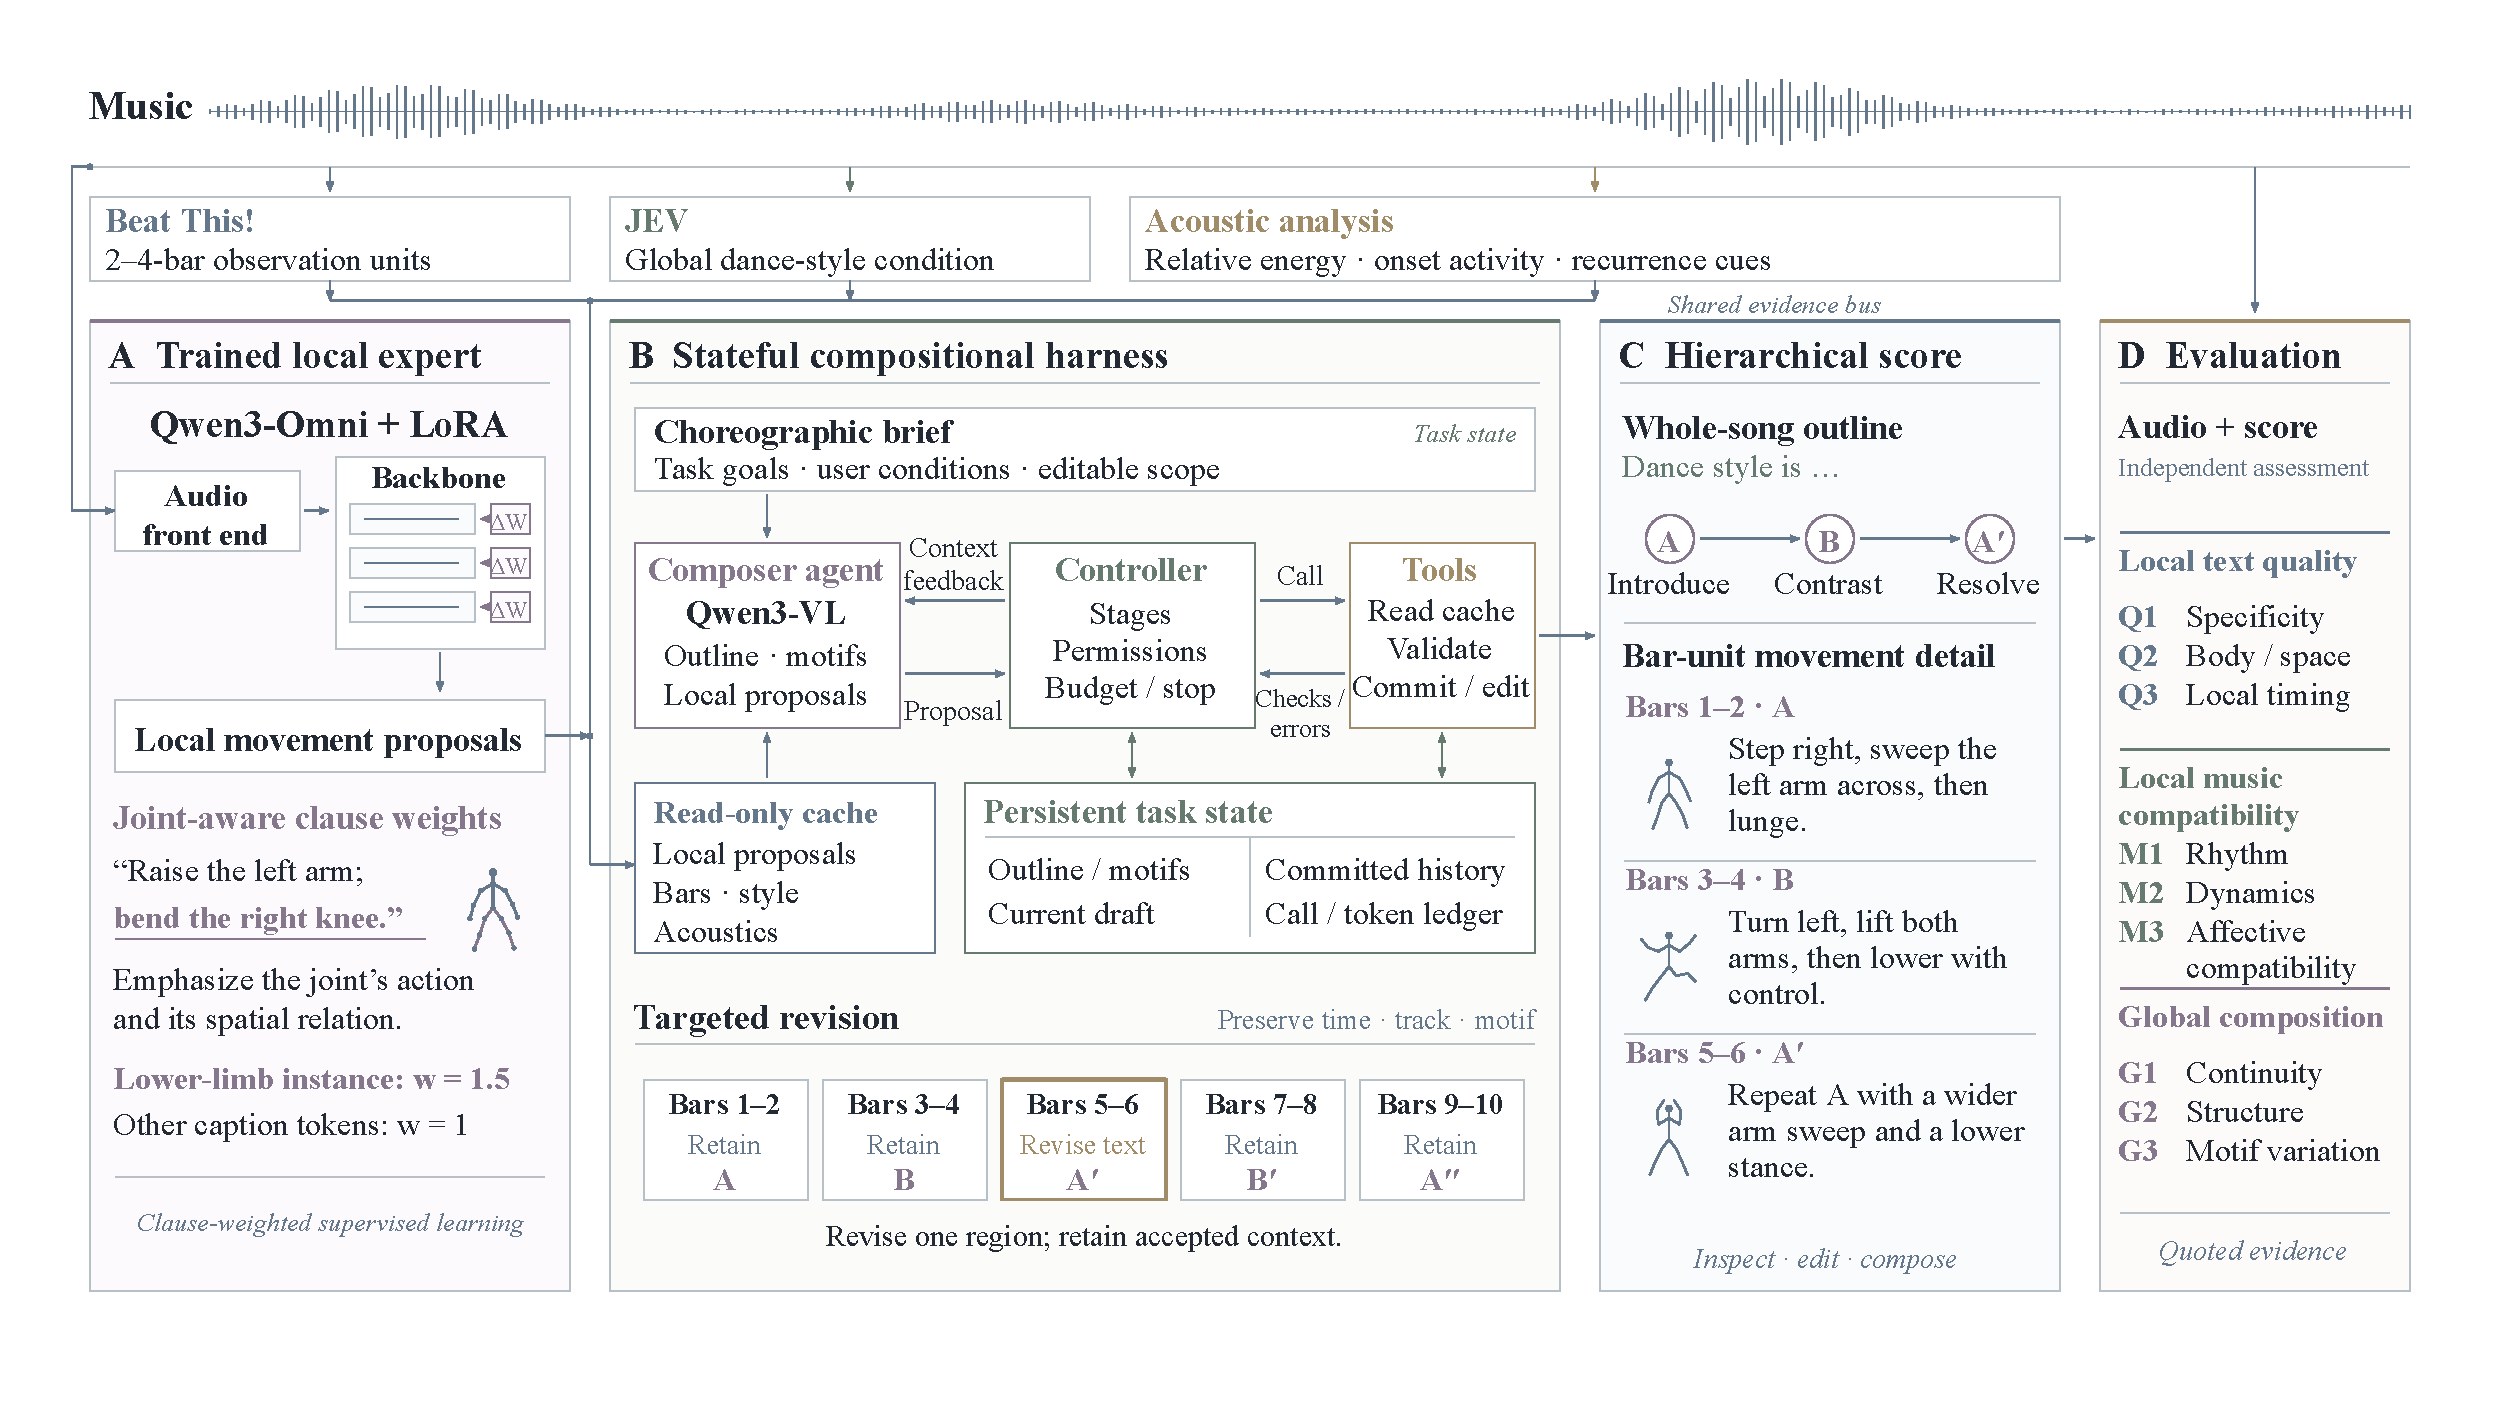
\includegraphics[width=\textwidth]{figures/revision_20261117/paper/overview_method.pdf}
\caption{\textbf{From a trained local expert to stateful composition.}
Joint-aware clause supervision trains our Qwen3-Omni expert; Beat This!,
JEV, and acoustic analysis provide shared musical conditions.
The composer proposes movements, the controller schedules tool
execution, and structural feedback informs subsequent decisions.
The task brief and persistent state retain objectives, drafts, motifs,
committed history, and budgets.
Targeted revision protects the temporal scaffold and accepted context.
The hierarchical score supports separate local and global assessment
outside the generation loop. Poses and score excerpts are schematic. The latest design uses bar
groups; reported whole-song results retain their fixed-window configuration.}
\fi
\label{fig:harness-overview}
\end{figure*}

